\documentclass{article}
\usepackage{graphicx} % Required for inserting images
\graphicspath{{Images/}}
\usepackage[utf8]{inputenc}
\usepackage{multicol}
\usepackage{amsthm}
\usepackage{amsmath}
\usepackage{xcolor}

\title{Analyse I - Théorèmes à l'examen}
\author{Laura Paraboschi - Simon Lefort}
\date{BA1 - Automne 2023}

\begin{document}

\maketitle

\section{Théorèmes à l'examen}

Ce document contient les énoncés et démonstrations des 12 théorèmes pouvant tomber à l'examen de janvier 2024 pour le cours d'analyse I de Adélie Garin (classe inversée). Rédigé par des BA1, donc à prendre avec du recul malgré toutes nos précautions ;)\\
Nous avons gardé la formulation utilisée dans les vidéos du professeur Peter Wittwer, dont sont tirées les quelques illustrations.

\newpage

\section{Mémos par théorèmes}

\textbf{unicité de la limite} $ \rightarrow $ par l'absurde, poser $ \frac{\epsilon}{2} N_{max}, a - b = (a - a_n) + (a_n - b)$\\\\
\textbf{théorème des gendarmes} $ \rightarrow $ poser encadrement, $ N_{max} $\\\\
\textbf{si une série converge, la suite des termes tend vers 0} $ \rightarrow $ suite des sommes partielles est de Cauchy\\\\
\textbf{prouver que la limite de f donnée est 0} $ \rightarrow $ rappeler la définition de la limite épointée et l'appliquer\\\\
\textbf{prouver que la lim de sin(1/x) en 0 n'existe pas} $ \rightarrow $ choisir deux suites $ \frac{1}{2n\pi} $ et $ \frac{1}{2n\pi + \frac{\pi}{2}}$ OU $ \frac{1}{n\pi + \frac{pi}{2}}$\\\\
\textbf{théorème des gendarmes pour les fonctions} $ \rightarrow $ deux suppositions, disjonctions de cas sur $ x^* $ jusqu'à redirection vers le théorème des gendarmes pour les suites\\\\
\textbf{théorème du point fixe} $ \rightarrow $ poser $ x - f(x) $\\\\
\textbf{dérivabilité implique continuité} poser $ \lim_{x\to{x_0}} (f(x) - f(x_0)) $, multiplier par $(x - x_0)$\\\\
\textbf{continuité et dérivabilité de $ f $ bijective implique $f^{-1}$ dérivable} utiliser la dérivation en chaîne et penser à $ f^{-1'}(x) \neq 0 $\\\\
\textbf{théorème des accroissements finis (TAF)} penser à Rolle et poser $g(x) = f(x) - (f(a) + \frac{f(b) - f(a)}{b - a}(x-a))$.\\\\
\textbf{TAF généralisé} penser à Rolle et poser $ h(x) = f(x) - (f(a) + \frac{f(b) - f(a)}{g(b) - g(a)}(g(x) - g(a)) $.\\\\
\textbf{théorème de la moyenne} penser au TVI et $ f(u) = \frac{1}{b-a} \cdot \int_{a}^{b} f(x)dx $\\\\
\textbf{théorème de la moyenne généralisé} penser au TVI et $ \int_{a}^b f(x)\cdot g(x)dx = f(u) \cdot \int_{a}^b g(x)dx $ + borner min max de f

\newpage

\section{Unicité de la limite d'une suite}

\subsection{Enoncé}

La limite d'une suite, si elle existe, est unique.

\subsection{Démonstration}

Supposons par l'absurde que:
\[ \lim_{n\to\infty}a_n = a\ \text{et} \lim_{n\to\infty}a_n = b,\ \text{avec a}\ \neq b \].\\
Alors:
\[ \lim_{n\to\infty}a_n = a\ \Leftrightarrow \forall \epsilon > 0,\ \exists n_1 \in \mathbf{N^*},\ \text{t.q.}\ \forall n > n_1,\ \lvert a_n - a \lvert\ \leq \frac{\epsilon}{2}\ \textbf{(1)}\]
\[ \lim_{n\to\infty}a_n = b\ \Leftrightarrow \forall \epsilon > 0,\ \exists n_2 \in \mathbf{N^*},\ \text{t.q.}\ \forall n > n_2,\ \lvert a_n - b \lvert\ \leq \frac{\epsilon}{2}\ \textbf{(2)}\]\\
Soit $ n_0 := max(n_1, n_2) $.\\
$ \forall n \geq n_0 $, on a à la fois \textbf{(1)} et \textbf{(2)}.\\
Puisque $ a - b = (a - a_n) + (a_n - b) $, alors $\forall \epsilon > 0, \forall n \geq n_0 $ :\\
\[ 0\ \leq \lvert a - b \lvert\ \leq \lvert a_n - a \lvert\ +\ \lvert a_n - b \lvert\ \leq \frac{\epsilon}{2} + \frac{\epsilon}{2} = \epsilon \]
\[ \Leftrightarrow 0 \leq |a-b| \leq \epsilon \]
\textit{petite note : $ |a - a_n| = |a_n - a|, $ propriétés de la valeur absolue.}\\\\
L'axiome d'Archimède nous permet d'affirmer que si $ p \in R\ \text{et}\ \forall \epsilon > 0 \in \mathbf{R},\ 0 \leq p \leq \epsilon \implies p = 0 $. \\\\
Ainsi, $ a - b = 0 $, donc $ a = b $ ce qui contredit notre supposition de départ.

\newpage

\section{Théorème des gendarmes}

\subsection{Enoncé}

\textbf{Hypothèses} \\
\[ \lim_{n\to\infty}a_n = \lim_{n\to\infty}b_n = c \]
\[ \exists m, \text{s.t } a_n < c_n < b_n\ \forall n \in \mathbf{N} \geq m \]
\textbf{Alors} \\
\[ \lim_{n\to\infty}c_n = c \]

\subsection{Démonstration}

On a $a_n \leq c_n \leq b_n \Leftrightarrow a_n - c \leq c_n - c \leq b_n - c \quad \forall n \geq m$ par l'hypothèse 2 \\
\begin{itemize}
    \item $\forall \epsilon > 0,\exists n_1 \in \mathbf{N}$ tel que $\forall n\geq n_1 \lvert a_n - c \lvert < \epsilon$ puisque $a_n$ converge
    \item $\forall \epsilon > 0,\exists n_2 \in \mathbf{N}$ tel que $\forall n\geq n_2 \lvert b_n - c \lvert < \epsilon$ puisque $b_n$ converge
\end{itemize}
Posons N = max($m$, $n_1, n_2)$, alors : \\\\
On a (1) : $a_n - c \leq c_n - c \leq b_n - c \quad \forall n \geq N$\\\\
On a (2) : $\forall \epsilon > 0, \forall n\geq N$
\begin{itemize}
    \item $ \lvert a_n - c \lvert < \epsilon \implies -\epsilon \leq a_n - c \leq \epsilon$
    \item $ \lvert b_n - c \lvert < \epsilon \implies -\epsilon \leq b_n - c \leq \epsilon$
\end{itemize}
Par la définition de la limite et de N, on obtient, $\forall n\geq N$ :
\[ -\epsilon \leq a_n - c \leq c_n - c \leq b_n - c \leq \epsilon  \]
\[ \implies -\epsilon\leq c_n - c \leq \epsilon \]
\[ \implies \lvert c_n - c \lvert < \epsilon \]
\[ \implies \lim_{n\to\infty}c_n = c \]

\newpage

\section{Si une série converge, la suite des termes tend vers 0}

On veut démontrer :
\[ \sum_{k=0}^{\infty} a_k\ \text{converge} \implies \lim_{n\to\infty} a_n = 0 \]\\
Une série est dite convergente si la suite des sommes partielles $S_n = \sum_{k=0}^{n} a_k$ converge vers une limite finie lorsque $n$ tend vers l'infini. Ainsi si la série est convergente, $ S_n $ est une suite de Cauchy.
alors :
\[ \forall \epsilon > 0,\ \exists\ N\ \text{t.q}\ \forall n, m \geq N \in \mathbf{N},\ \lvert S_n - S_m \lvert\ \leq \epsilon \]
en particulier, on a :
\[ \lvert S_{m+1} - S_m \lvert\ \leq \epsilon \]
\[ \Leftrightarrow \lvert a_{m+1} \lvert\ \leq \epsilon \]\\\\
Ainsi, on retrouve la définition de limite pour $ a_n $:\\
\[ \forall\ \epsilon > 0,\ \exists\ n_0 \in \mathbf{N},\ \text{t.q}\ \forall n \geq n_0 + 1,\ |a_n - 0| \leq \epsilon \]
\[ \Leftrightarrow \lim_{n\to\infty} a_n = 0 \]

\newpage

\section{Prouver que la limite d'une fonction f donnée est 0}

\subsection{Enoncé}
On nous donne la suite $ f(x) = 0 $ si $ x \neq 0 $, et $ f(0) = 1 $.\\
On veut démontrer que $ \lim_{x\to{0}} f(x) = 0 $. (et non pas 1...)
\subsection{Définition de la limite épointée :}
$ f : D \to \mathbf{R} $ admet pour limite épointée $ l \in \mathbf{R} $ lorsque $ x \to x^* $ si :\\
$ \forall (x_n) $ t.q
\begin{itemize}
    \item $\forall n, x_n \in D \backslash \{x^*\} $
    \item $ \lim_{n\to\infty} x_n = x^*$
\end{itemize}
alors la suite $ y_n = f(x_n) $ converge et $ \lim_{n\to\infty} y_n = l$

\subsection{Démonstration}
Ici notre $ x^* = 0 $, donc on choisit une suite $ x_n $ telle que $ \lim_{n\to\infty} x_n = 0$, et $ x_n \neq 0$ (ex $\frac{1}{n}$). On a donc $ \forall n, y_n = f(x_n) = 0 $ car $x_n \neq 0$.\\\\
Ainsi, on peut connaître $ \lim_{n\to\infty} y_n = l = \lim_{n\to\infty} 0 = 0$.

\newpage
\section{Prouver que la limite de $ sin(\frac{1}{x}) $ en 0 n'existe pas}

\subsection{Enoncé}
On nous donne la fonction $ f(x) = sin(\frac{1}{x}) $.\\
On veut démontrer que $ \lim_{x\to{0}} f(x) $ n'existe pas
\subsection{Définition de la limite épointée :}
$ f : D \to \mathbf{R} $ admet pour limite épointée $ l \in \mathbf{R} $ lorsque $ x \to x^* $ si :\\
$ \forall (x_n) $ t.q
\begin{itemize}
    \item $\forall n, x_n \in D \backslash \{x^*\} $
    \item $ \lim_{n\to\infty} x_n = x^*$
\end{itemize}
alors la suite $ y_n = f(x_n) $ converge et $ \lim_{n\to\infty} y_n = l$
\subsection{Démonstration}
Ici notre $ x^* = 0 $. 
\subsubsection{Méthode 1}
On doit trouver une suite $ x_n $ t.q $ \lim_{n\to\infty}x_n= 0 $ et $ x_n \neq 0$, mais t.q $ y_n = f(x_n) $ diverge.\\\\
On pose $ x_n = \frac{1}{\frac{\pi}{2} + n \cdot \pi}$. On a $ y_n = sin(\frac{\pi}{2} + f+n \cdot \pi) = (-1)^n $ qui ne converge pas.
\subsubsection{Méthode 2}
On trouve deux suites $x_n$, $z_n$ telle que $y_n$ diverge : \\\\
$x_n = \frac{1}{2\pi n}$ et $z_n = \frac{1}{\frac{\pi}{2} + 2\pi{n}}$ \\\\
On a $x_n = 0,\ z_n = 0,\ \lim_{n\to\infty}x_n = 0\ et \lim_{n\to\infty}z_n = 0$ \\\\
$y_n = f(x_n) = sin(2\pi n) = 0,\ y_{n2} = f(z_n) = sin(\frac{\pi}{2} + 2\pi n) = 1$ \\\\
donc $\lim_{n\to\infty}y_n = 0$ mais $\lim_{n\to\infty}y_{n2} = 1$

\newpage
\section{Théorème des deux gendarmes pour les fonctions}

\subsection{Enoncé}

Soient $ f, g, h: D \to \mathbf{R}, D \subset \mathbf{R}, D \neq \emptyset $\\
Soit $ x^* \in \mathbf{R} $ ou $ x^* \in \{-\infty, +\infty\}$\\\\
Supposons :

\paragraph{i)}

\begin{itemize}
    \item cas $ x^* \in \mathbf{R} $ :

$ \exists \epsilon > 0 $ t.q $ \forall x \in D $, $ |x-x^*| \leq \epsilon \implies f(x) \leq g(x) \leq h(x) $

\item cas $ x^* = +\infty $ :

$ \exists \epsilon > 0 $ t.q $ \forall x \in D $, $ x > \epsilon \implies f(x) \leq g(x) \leq h(x) $

\item cas $ x^* = -\infty $ :

$ \exists \epsilon < 0 $ t.q $ \forall x \in D $, $ x < \epsilon \implies f(x) \leq g(x) \leq h(x) $

\end{itemize}

\paragraph{ii)}

$ \lim_{x\to{x^*}} f(x) = \lim_{x\to{x^*}} h(x) = l \in \mathbf{R} $\\\\
Alors : 

\[ \lim_{x\to{x^*}} g(x) = l \]

\subsection{Démonstration}

$ \epsilon $ est déterminé en fonction du cas dans i).\\
Soit une suite $ (x_n), x_n \in D, x_n \neq x^* $ et $ \lim_{n\to\infty} x_n = x^* $.\\\\
Par définition de $ \lim_{n\to\infty} x_n = x^*, \exists n_0 $, t.q, $ \forall n \geq n_0, $ :
\begin{itemize}
    \item $ |x_n - x^*| \leq \epsilon $ (cas où $ x^* \in \mathbf{R} $)
    \item $ x_n \geq \epsilon $ (cas où $ x^* = +\infty)$
    \item $ x_n \leq \epsilon $ (cas où $ x^* = -\infty)$
\end{itemize}
donc $ \forall n \geq n_0 $:
\[ f(x_n) \leq g(x_n) \leq h(x_n) \]
et par ii), $ \lim_{n\to\infty} f(x_n) = l $ et $ \lim_{n\to\infty} h(x_n) = l $, donc $ \lim_{n\to\infty} g(x_n) = l $ (par le théorème des gendarmes pour les suites).

\newpage

\section{Théorème du point fixe}

\subsection{Rappel : TVI}

Soit $ a, b \in \mathbf{R},\ a < b $. Toute fonction continue $ f : [a, b] \to \mathbf{R} $ prend (au moins une fois) toutes les valeurs entre f(a) et f(b).

\subsection{Enoncé}

\paragraph{Définition} : une fonction $ f : D \to \mathbf{R} $ admet $ x \in D $ comme point fixe si $ f(x) = x $.\\\\
Soit $ a, b \in \mathbf{R}, a < b $. Alors toute fonction continue $ f : [a, b] \to Im(f) \subset [a, b] $ admet un point fixe.\\\\

\begin{figure}[htp]
    \centering
    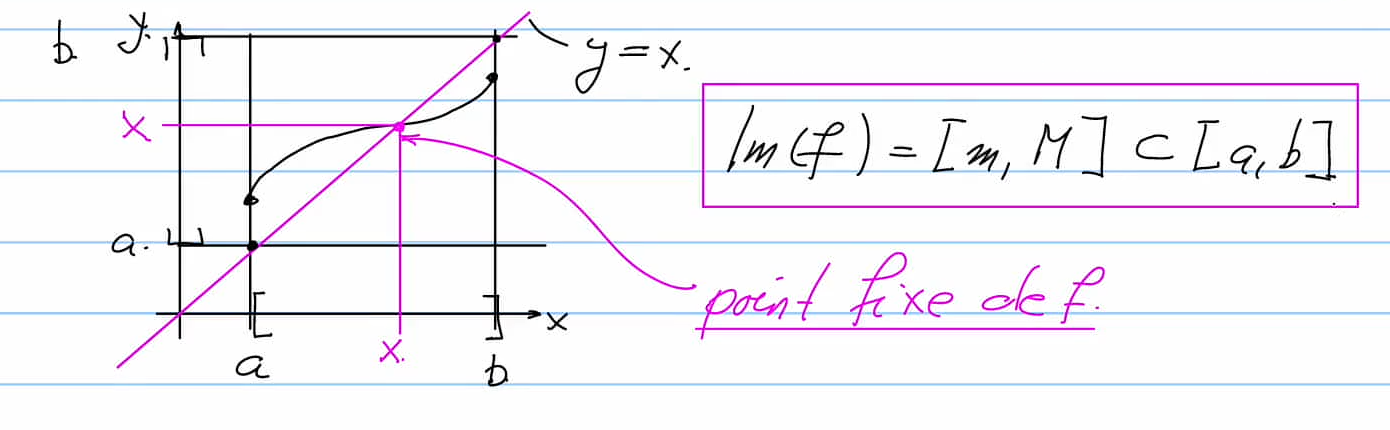
\includegraphics[width=12cm]{Images/pointfixe.png}
    \caption{Illustration du théorème du point fixe}
    \label{fig:complex}
\end{figure} 

\subsection{Démonstration}

Soit $ m $ le minimum de $ f(x) $. Comme $ Im(f) \subset [a, b] $, alors m $ \geq a $.\\
Soit $ M $ le maximum de $ f(x) $. Comme $ Im(f) \subset [a, b] $, alors M $ \leq b $.\\\\
La fonction $ g(x) := x - f(x) $ est continue sur $ [a, b] $ car $ f $ continue sur $ [a, b] $.
\[ g(a) = a - f(a) \leq a - a \leq 0 \]
\[ g(b) = b - f(b) \geq b - b \geq 0 \]
Par le théorème des valeurs intermédiaires $ \exists u \in [a, b] $ t.q $ g(u) = 0 \Leftrightarrow f(u) = u $.

\paragraph{Remarque}: pour les suites définies par récurrence par une fonction continue, ce théorème permet d'identifier les limites éventuelles.

\newpage

\section{Dérivabilité en $x_0$ implique continuité en $x_0$}

\subsection{Enoncé}

Une fonction qui est dérivable en $x_0$ est continue en $x_0$.

\subsection{Démonstration}

\[ \lim_{x\to{x_0}} (f(x) - f(x_0)) \]
\[ = \lim_{x\to{x_0}} \frac{f(x) - f(x_0)}{x-{x_0}} \cdot (x-{x_0}) \] (car limite épointée $ x \neq x_0 $)
\[ = \lim_{x\to{x_0}} \frac{f(x) - f(x_0)}{x-{x_0}} \cdot \lim_{x\to{x_0}} (x-{x_0})\] (en supposant que les deux limites existent séparément)
\[ = d \cdot 0 \]
\[ = 0 \]

donc $ \lim_{x\to{x_0}} f(x) = f(x_0) $ donc la fonction est continue.
\paragraph{Remarque}: la réciproque du théorème est fausse. Par exemple, $ f(x) = |x| $.

\newpage

\section{Continuité et dérivabilité de la fonction réciproque}

\subsection{Quelques rappels pour l'intuition}


\begin{itemize}
    \item toute fonction strictement monotone est injective :\\
$ x_1 < x_2 \implies f(x_1) < (\textbf{ou} >) f(x_2) $, donc $ f(x_1) \neq f(x_2) $ (injectivité).
    \item si une fonction $ f: D(f) \to Im(f) $ est injective, alors elle est bijective et on a la fonction réciproque $ f^{-1} : Im(f) \to D(f) $.
\end{itemize}

\subsection{Enoncé}

La réciproque d'une fonction bijective continue est continue sur l'image de tout intervalle.\\\\
La réciproque d'une fonction bijective dérivable est dérivable sur l'image de tout intervalle $ I $ \textbf{tel que $ \forall x \in I,\ f'(x) \neq 0 $} \textit{condition importante, voir $ f(x) = x^3 $}.\\\\
Soit I un intervalle, $ I \neq 0, f : I \to Im(f) \subset \mathbf{R} $ bijective, dérivable, $ \forall x \in I, f'(x) \neq 0 $. Alors :
\[ \forall y \in Im(f) = D(f^{-1}),\ f(^{-1})^{'}(y) = \frac{1}{f'(f^{-1}(y)} \]

\subsection{Démonstration}

Soit $ y = f(x) \Leftrightarrow x = f^{-1}(y) $.\\
On a donc $ \forall y \in D(f^{-1}) = Im(f),\ f(f^{-1}(y)) = y $.\\\\
Par dérivation en chaîne on obtient, $ \forall y \in Im(f) $ :
\[ f'(f^{-1}(y)) \cdot (f^{-1})'(y) = 1. \]
\[ \Leftrightarrow \ (f^{-1})'(y) = \frac{1}{f'(f^{-1}(y))}. \]

\newpage

\section{Théorème des accroissements finis}

\subsection{Rappel : Théorème de Rolle}

Soit $ f : D \to \mathbf{R}, [a,b] \subset D, a, b \in \mathbf{R}, a < b $, f continue sur $ [a, b] $ et dérivable sur $]a, b[$.\\\\
Si $ f(a) = f(b) = 0 $, alors il existe $ u \in ]a, b[ $ tel que $ f'(u) = 0 $.

\subsection{Enoncé}

Soit $ f : D \to \mathbf{R}, [a,b] \subset D, a, b \in \mathbf{R}, a < b $, f continue sur $ [a, b] $ et dérivable sur $]a, b[$.\\\\
Alors $ \exists u \in ]a, b[$ t.q:\\\\
$ f'(u) = \frac{f(b) -f(a)}{b - a}$(*)\\\\
\begin{figure}[htp]
    \centering
    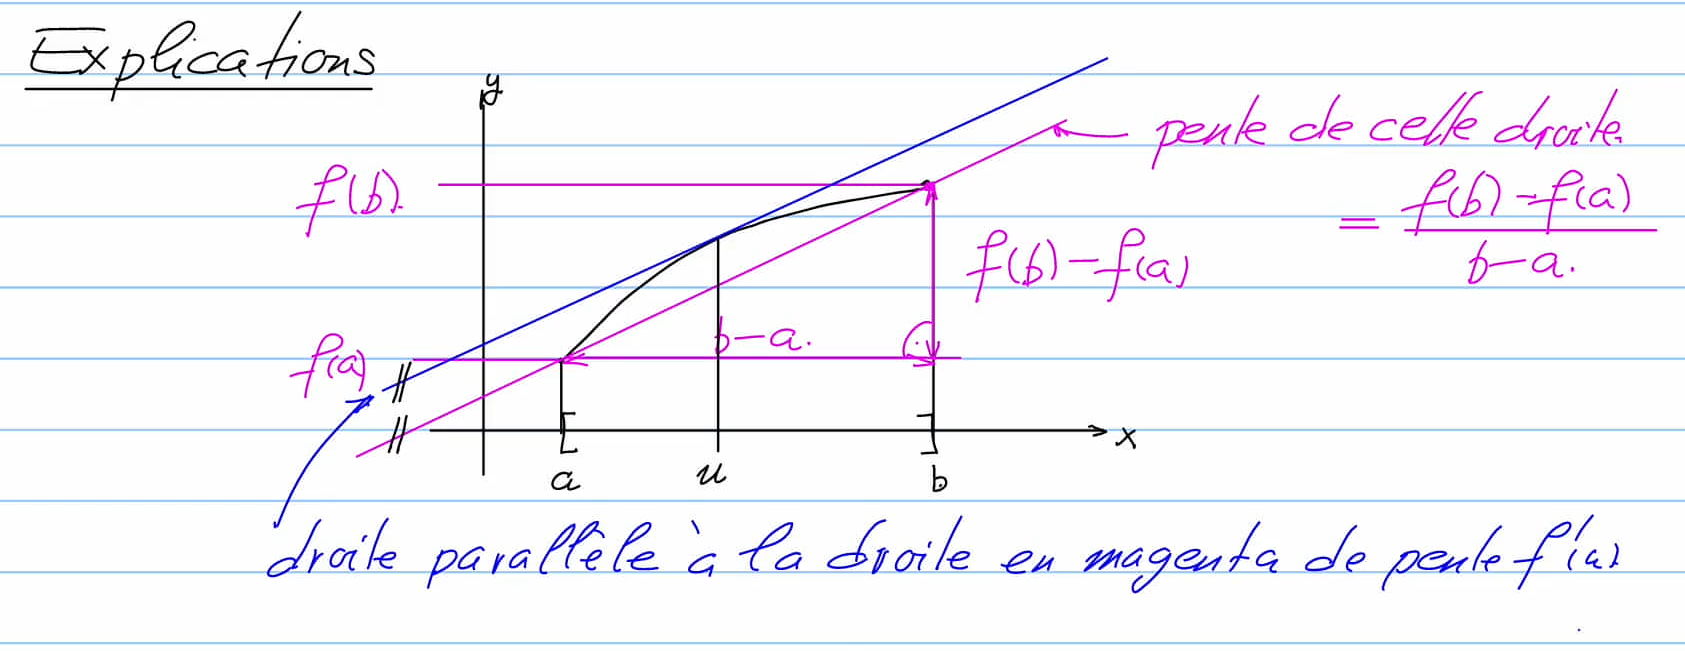
\includegraphics[width=8cm]{Images/accroissements.png}
    \caption{Théorème des accroissements finis}
\end{figure}

\subsection{Démonstration}

Soit $ g(x) = f(x) - (f(a) + \frac{f(b) - f(a)}{b - a}(x-a))$.\\\\
On choisit cette fonction pour que quand x = a ou x = b, on obtienne 0.\\\\
$ g(a) = f(a) - f(a) = 0 $\\
$ g(b) = f(b) - f(b) = 0 $\\
Comme $f$ est continue et dérivable sur $ ]a, b[$, g est aussi continue et dérivable sur ce même intervalle. Par le théorème de Rolle, $ \exists u \in ]a, b[ $ t.q $ g'(u) = 0 = f'(u) - (0 + \frac{f(b) - f(a)}{b - a}) \implies *$.

\newpage

\section{Théorème des accroissements finis généralisés}

\subsection{Enoncé}

Soient 
\begin{itemize}
    \item $ f : D(f) \to \mathbf{R} $
    \item $ g : D(g) \to \mathbf{R} $
    \item $ a, b \in \mathbf{R}, a < b $
\end{itemize}
Par hypothèse:
\begin{itemize}
    \item $ [a,b] \subset D(f) \cap D(g) $
    \item $ f, g $ continues sur $ [a, b] $
    \item $ f, g $ dérivables sur $ ]a, b[ $
    \item $ \forall x \in\ ]a, b[,\ g'(x) \neq 0. $
\end{itemize}
Alors il existe $ u \in ]a, b[ $, tel que :
\[ \frac{f'(u)}{g'(u)} = \frac{f(b) - f(a)}{g(b) - g(a)}\]
Remarque : pour $ g(x) = x $ c'est le théorème des accroissements finis.\\
Remarque : $ \forall x \in ]a, b[, g'(x) \neq 0 \implies g(b) \neq g(a)$

\subsection{Démonstration}

"On se bricole une fonction qui a toutes les propriétés requises."\\\\
On pose :\\
$ h(x) = f(x) - (f(a) + \frac{f(b) - f(a)}{g(b) - g(a)}(g(x) - g(a)) $\\
On a $ h(a) = h(b) = 0 $, et on applique le théorème de Rolle.

\newpage

\section{Théorème de la moyenne}

\subsection{Enoncé}

Soient 

\begin{itemize}
    \item $ f: D \to R $
    \item $ a < b \in \mathbf{R} $
    \item $ [a, b] \subset D $
    \item $ f $ continue sur $ [a, b]\ (\Leftrightarrow f \in C^0([a, b])) $
\end{itemize}
Alors, grâce au T.V.I (voir schéma), on sait qu'il existe $ u \in ]a, b[$ tel que:
\[ \int_{a}^bf(x)dx = f(u)(b - a) = f(u) \cdot \int_{a}^b 1\cdot dx \]
Remarque : $f(u)$ est la valeur moyenne de la fonction entre a et b
\[ f(u) = \frac{1}{b-a} \cdot \int_{a}^{b} f(x)dx \]
\begin{figure}[htp]
    \centering
    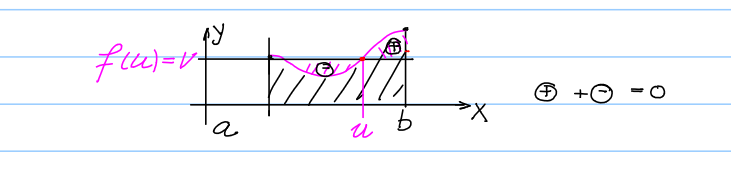
\includegraphics[width=0.8\linewidth]{Images/moyenne.png}
    \caption{Illustration du théorème de la moyenne}
    \label{fig:enter-label}
\end{figure}

\subsection{Enoncé (Généralisation)}

Soient :
\begin{itemize}
    \item $ f, g $ continues sur $ [a, b]\ (\Leftrightarrow \in C^0([a, b]) $
    \item $ \forall x \in [a, b],\  g(x) > 0 $
\end{itemize}
Alors il existe $ u \in ]a, b[ $ tel que:
\[ \int_{a}^b f(x)\cdot g(x)dx = f(u) \cdot \int_{a}^b g(x)dx \]

\newpage

\subsection{Démonstration}

Soient $ m $ et $ M $ le minimum et le maximum de $ f $ sur $ [a, b] $. Comme $ g(x) > 0 $ alors:

\[ \forall x \in [a, b],\ m \leq f(x) \leq M \]
\[ \Leftrightarrow \forall x \in [a, b],\ m \cdot g(x) \leq f(x) \leq M \cdot g(x) \]
on applique les propriétés de l'intégrale:
\[ m \cdot \int_{a}^b g(x)dx \leq \int_{a}^b f(x)g(x)dx \leq M \cdot \int_{a}^b g(x)dx \]
Et il existe donc $ v \in [m, M] $ tel que:
\[ \int_{a}^b f(x)g(x)dx = f(v) \cdot \int_{a}^b g(x)dx \]
On peut prouver qu'il existe un tel $ v $ car $ f $ est continue, grâce au T.V.I, $ \exists u \in ]a, b[ $ tel que $ v = f(u) $.

\end{document}
